\documentclass{article}

\usepackage{graphicx}
\usepackage{tikz}
\usepackage{tikzsymbols}
\usetikzlibrary{calc,patterns,shapes.geometric}
\pagestyle{empty}
\usepackage[margin=0pt]{geometry}
\geometry{papersize={14in,12in}}

\def\centerarc[#1](#2)(#3:#4:#5){\draw[#1] ($(#2)+({#5*cos(#3)},{#5*sin(#3)})$) arc (#3:#4:#5);}

\begin{document}
	\begin{figure}
		\centering
		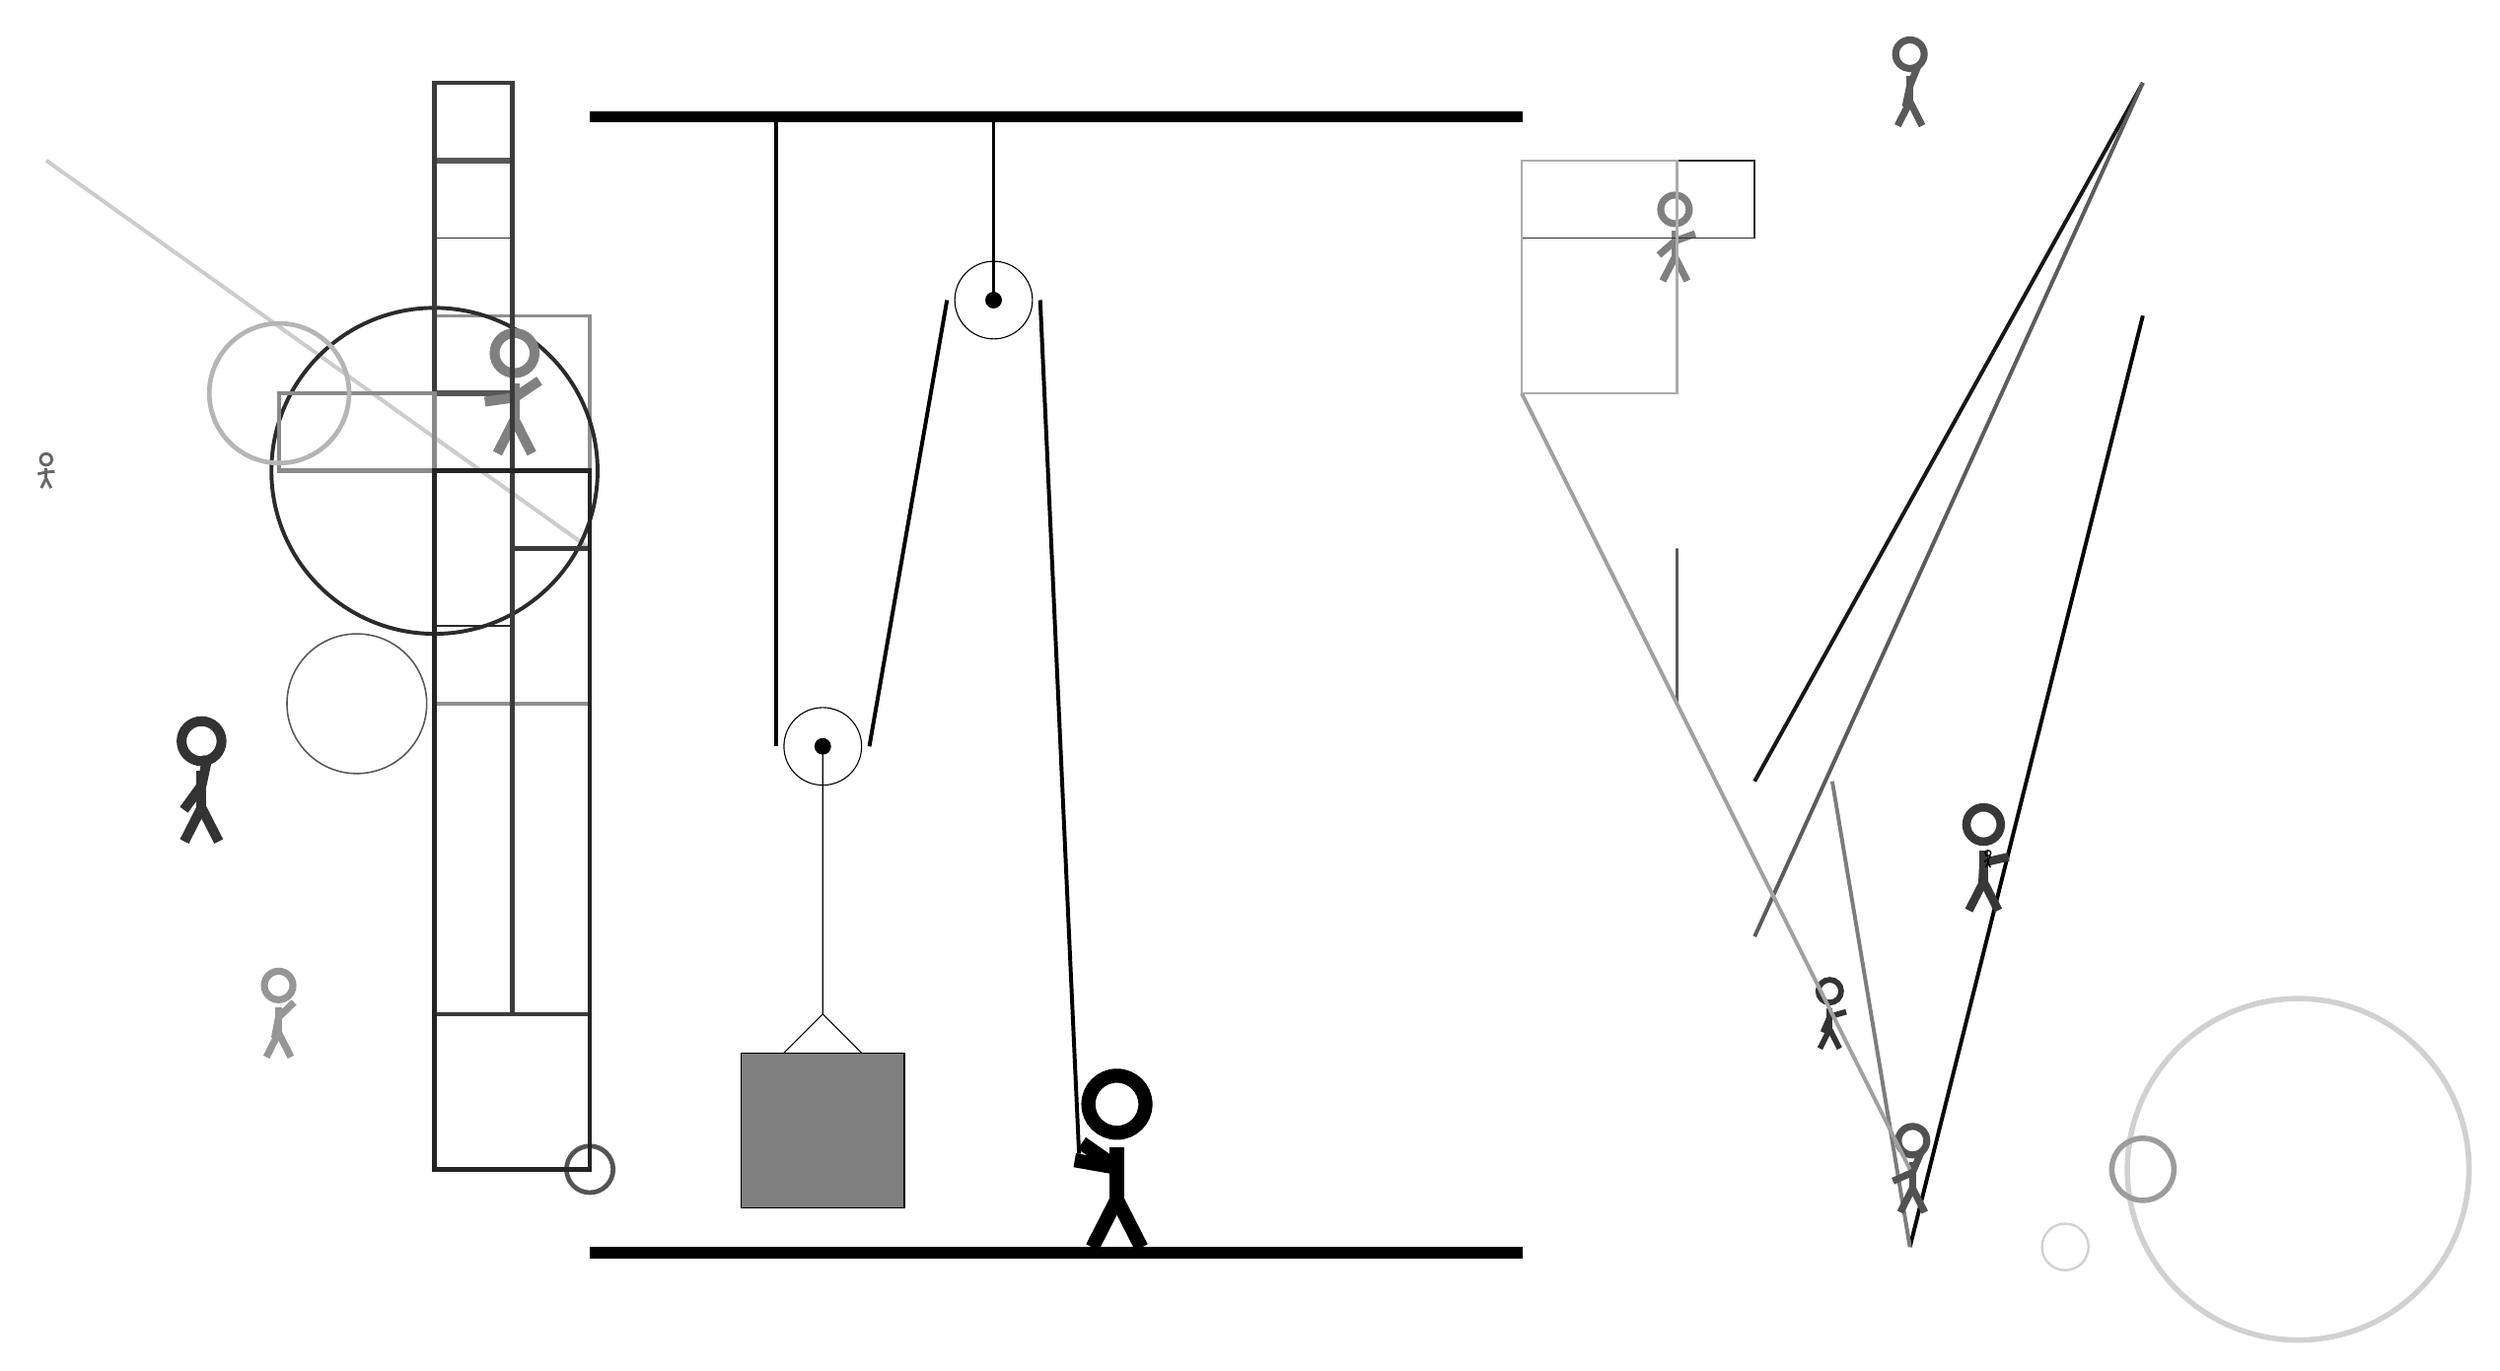
\begin{tikzpicture}
			%%%%% START %%%%%
			
			\draw[fill=black] (-2, 11.5) rectangle (10, 11.625);
			
			\draw (3.2, 9.2) circle (0.5);
			\draw[fill=black] (3.2, 9.2) circle (0.1);
			\draw[thick] (3.2, 9.2) -- (3.2, 11.5);
			
			\draw[line width=0.3mm, color=black!65] (12, 6) rectangle (12, 4);
			
			\draw[line width=0.4mm, color=black!44] (-2, 4) rectangle (-4, 9);
			\node[line width=0.5mm, color=black!80] at (14, 0) {\Strichmaxerl[4][67][16]};
			\node[line width=0.5mm, color=black!60] at (-9, 7) {\Strichmaxerl[2][13][4]};
			\draw[line width=0.5mm, color=black!91](13, 3) -- (18, 12);
			
			\node[line width=0.2mm, color=black!50] at (12, 10) {\Strichmaxerl[5][41][20]};
			
			\draw[line width=0.5mm, color=black!64](13, 1) -- (18, 12);
			\draw[line width=0.5mm, color=black!20](-2, 6) -- (-9, 11);
			\node[line width=0.6mm, color=black!65] at (15, 12) {\Strichmaxerl[5][78][68]};
			
			\draw [line width=0.7mm, color=black!18](20, -2) circle (2.2);
			
			\node[line width=0.7mm, color=black!80] at (-7, 3) {\Strichmaxerl[7][54][78]};
			\draw [line width=0.6mm, color=black!67](-2, -2) circle (0.3);
			\draw[line width=0.5mm, color=black!98](15, -3) -- (18, 9);
			
			\draw [line width=0.5mm, color=black!83](-4, 7) circle (2.1);
			\draw[line width=0.7mm, color=black!66] (-4, 11) rectangle (-3, 8);
			\draw[line width=0.2mm, color=black!83] (10, 11) rectangle (13, 10);
			
			\node[line width=0.3mm, color=black!41] at (-6, 0) {\Strichmaxerl[5][79][44]};
			
			\node[line width=0.2mm, color=black!50] at (-3, 8) {\Strichmaxerl[7][8][34]};
			\draw [line width=0.3mm, color=black!18](17, -3) circle (0.3);
			\node[line width=0.7mm, color=black!78] at (16, 2) {\Strichmaxerl[6][87][13]};
			\draw[line width=0.5mm, color=black!51](15, -3) -- (14, 3);
			
			\draw[line width=0.2mm, color=black!84] (-3, 5) rectangle (-4, 10);
			\draw[line width=0.6mm, color=black!77] (-3, 0) rectangle (-2, 6);
			\node[line width=0.3mm, color=black!68] at (15, -2) {\Strichmaxerl[5][24][67]};
			\draw[line width=0.6mm, color=black!77] (-4, 12) rectangle (-3, 0);
			
			\node[line width=0.2mm, color=black!100] at (16, 2) {\Strichmaxerl[1][29][55]};
			
			\draw[line width=0.5mm, color=black!37](10, 8) -- (15, -2);
			\draw[line width=0.6mm, color=black!46] (-4, 8) rectangle (-6, 7);
			\draw[line width=0.3mm, color=black!32] (10, 11) rectangle (12, 8);
			\draw[line width=0.6mm, color=black!86] (-4, -2) rectangle (-2, 7);
			\draw [line width=0.6mm, color=black!29](-6, 8) circle (0.9);
			
			\draw [line width=0.7mm, color=black!39](18, -2) circle (0.4);
			\draw [line width=0.2mm, color=black!65](-5, 4) circle (0.9);
			
			\draw (1, 3.45) circle (0.5);
			\draw[fill=black] (1, 3.45) circle (0.1);
			
			\draw (1, 3.45) -- (1, 0.0) -- (0.5, -0.5);
			\draw (1, 0.0) -- (1.5, -0.5);
			\draw[fill=black!50] (-0.05, -0.5) rectangle (2.05, -2.5);
			
			\draw[line width=0.5mm] (0.4, 11.5) -- (0.4, 3.45);
			\centerarc[line width=0.5mm](1, 3.45)(180:360:0.6);
			\draw[line width=0.5mm](1.6, 3.45) -- (2.6, 9.2);
			\centerarc[line width=0.5mm](3.2, 9.2)(0:180:0.6);
			\draw[line width=0.5mm](3.8, 9.2) -- (4.3, -1.8);
			
			\node at (4.7, -1.9) {\Strichmaxerl[10][-35][170]};
			
			\draw[fill=black] (-2, -3) rectangle (10, -3.15);
			
			%%%%% END %%%%%
		\end{tikzpicture}
	\end{figure}	
\end{document}